\documentclass[a4paper, 12pt]{article}

\def\languages{french, english}

%%%%%%%%%%%%%%%%%%% Libraries

%%%%%%%%%% Packages

\usepackage[
backend=biber,
style=numeric-comp,
sorting=none,
maxbibnames=99
]{biblatex}

\newgeometry{margin = 2.5cm}
\makeatletter
\begin{titlepage}
	\begin{minipage}[t][0.425\textheight][t]{\textwidth}
		\begin{center}
		    \ifx\toptitle\undefined
    		    \vfill
    		    \ifx\logopath\undefined
    		    \else
    			    \includegraphics[height=0.2125\textheight]{\logopath}
    			\fi
    		\else
    		    \ifx\logopath\undefined
    		    \else
    			    \includegraphics[height=0.15\textheight]{\logopath}
    			\fi
    			\vfill
    			{\huge \textsc{\toptitle}}
			\fi
			\vfill
		\end{center}
	\end{minipage}
	\vfill
	\begin{minipage}{\textwidth}
		\hspace{0.5em}
		\begin{mdframed}[linewidth = 2pt, innertopmargin = 1em, innerbottommargin = 1em, leftline = false, rightline = false]
			\begin{center}
				{\huge \bfseries \@title}
			\end{center}
		\end{mdframed}
		\hspace{0.5em}
	\end{minipage}
	\vfill
	\begin{minipage}[b][0.425\textheight][t]{\textwidth}
			\ifx\subtitle\undefined
			\else
			    \vspace{-1em}
			    \begin{center}
				    {\LARGE \subtitle}
				\end{center}
			\fi
			\vfill
			\ifx\rightauthor\undefined
			    \begin{center}
			        \ifx\authorhead\undefined
			        \else
		                {\large\it \authorhead\\[0.5em]}
		            \fi
			        {\large \@author}
			    \end{center}
			\else
			    \begin{minipage}[t]{0.5\textwidth}
			        \begin{flushleft}
			            \ifx\authorhead\undefined
			            \else
			                {\large\it \authorhead\\[0.5em]}
			            \fi
				        {\large \@author}
				    \end{flushleft}
				\end{minipage}
				\begin{minipage}[t]{0.5\textwidth}
				    \begin{flushright}
				        \ifx\rightauthorhead\undefined
			            \else
			                {\large\it \rightauthorhead\\[0.5em]}
			            \fi
				        {\large \rightauthor}
				    \end{flushright}
				\end{minipage}
			\fi
			\vfill
			\begin{center}
			    \ifx\context\undefined
			    \else
			        {\large \context \\[0.5em]}
			    \fi
			    {\large \@date}
			\end{center}
	\end{minipage}
\end{titlepage}
\makeatother
\restoregeometry
%%%%%%%%%% Packages

\usepackage{float}
\usepackage[skip=1em]{caption}
\usepackage{subcaption}

\usepackage{array}
\usepackage{multirow}
\usepackage{multicol}

%%%%%%%%%% Features

%%%%% Settings

\renewcommand{\arraystretch}{1.2}

%%%%% Commands

\newcommand\noskipcaption[1]{\caption{#1}\vspace{-1em}}
\newcommand\noskipcaptionstar[1]{\caption*{#1}\vspace{-1em}}

%%%%%%%%%% Packages

\usepackage{amsmath}
\usepackage{amssymb}
\usepackage{bm}
\usepackage{esint}
\usepackage[makeroom]{cancel}

%%%%%%%%%% Features

%%%%% Macros

\newcommand{\rbk}[1]{\left(#1\right)}
\newcommand{\cbk}[1]{\left\{#1\right\}}
\newcommand{\sbk}[1]{\left[#1\right]}
\newcommand{\abs}[1]{\left|#1\right|}
\newcommand{\norm}[1]{\left\|#1\right\|}

\newcommand{\fact}[1]{#1!}
\newcommand{\e}[1]{\mathbf{e}_{#1}}
\newcommand{\deriv}{\mathrm{d}}
\DeclareMathOperator{\tr}{tr}

\def\Rl{\mathbb{R}}
\def\Cx{\mathbb{C}}
\def\Na{\mathbb{N}}
\def\Zi{\mathbb{Z}}

%%%%%%%%%% Packages

\usepackage{siunitx}

%%%%%%%%%% Features

%%%%% Settings

\ifx\decimalsign\undefined
\else
    \sisetup{output-decimal-marker = \decimalsign}
\fi


%%%%%%%%%%%%%%%%%%% Bibliography

\addbibresource{resources/bib/ref.bib}

%%%%%%%%%%%%%%%%%%% Titlepage

\def\logopath{./resources/pdf/logo.pdf}
\def\toptitle{University of Liège}
\title{Project 1}
\def\subtitle{\textsc{INFO0009} - Bases des données (Databases)}
%\def\authorhead{}
\author{
Yusuf \textsc{Agirbas} (s225049)\\
Ibrahim \textsc{Touhami} (s220915) \\
Duy Vu \textsc{Dinh} (s2401627)\\
}
%\def\rightauthorhead{}
%\def\rightauthor{}
% \def\context{MSc in Data science and engineering}
\date{Année académique 2024-2025}
%%%%%%%%%%%%%%%%%%%

\usepackage{mhchem}
\usepackage{wrapfig}
\usepackage{xcolor}

\usepackage{pdflscape}

%%%%%%%%%%%%%%%%%%%

\begin{document}
\newgeometry{margin = 2.5cm}
\makeatletter
\begin{titlepage}
	\begin{minipage}[t][0.425\textheight][t]{\textwidth}
		\begin{center}
		    \ifx\toptitle\undefined
    		    \vfill
    		    \ifx\logopath\undefined
    		    \else
    			    \includegraphics[height=0.2125\textheight]{\logopath}
    			\fi
    		\else
    		    \ifx\logopath\undefined
    		    \else
    			    \includegraphics[height=0.15\textheight]{\logopath}
    			\fi
    			\vfill
    			{\huge \textsc{\toptitle}}
			\fi
			\vfill
		\end{center}
	\end{minipage}
	\vfill
	\begin{minipage}{\textwidth}
		\hspace{0.5em}
		\begin{mdframed}[linewidth = 2pt, innertopmargin = 1em, innerbottommargin = 1em, leftline = false, rightline = false]
			\begin{center}
				{\huge \bfseries \@title}
			\end{center}
		\end{mdframed}
		\hspace{0.5em}
	\end{minipage}
	\vfill
	\begin{minipage}[b][0.425\textheight][t]{\textwidth}
			\ifx\subtitle\undefined
			\else
			    \vspace{-1em}
			    \begin{center}
				    {\LARGE \subtitle}
				\end{center}
			\fi
			\vfill
			\ifx\rightauthor\undefined
			    \begin{center}
			        \ifx\authorhead\undefined
			        \else
		                {\large\it \authorhead\\[0.5em]}
		            \fi
			        {\large \@author}
			    \end{center}
			\else
			    \begin{minipage}[t]{0.5\textwidth}
			        \begin{flushleft}
			            \ifx\authorhead\undefined
			            \else
			                {\large\it \authorhead\\[0.5em]}
			            \fi
				        {\large \@author}
				    \end{flushleft}
				\end{minipage}
				\begin{minipage}[t]{0.5\textwidth}
				    \begin{flushright}
				        \ifx\rightauthorhead\undefined
			            \else
			                {\large\it \rightauthorhead\\[0.5em]}
			            \fi
				        {\large \rightauthor}
				    \end{flushright}
				\end{minipage}
			\fi
			\vfill
			\begin{center}
			    \ifx\context\undefined
			    \else
			        {\large \context \\[0.5em]}
			    \fi
			    {\large \@date}
			\end{center}
	\end{minipage}
\end{titlepage}
\makeatother
\restoregeometry

\newpage


\begin{landscape}

\begin{figure}[ht]
    \centering
    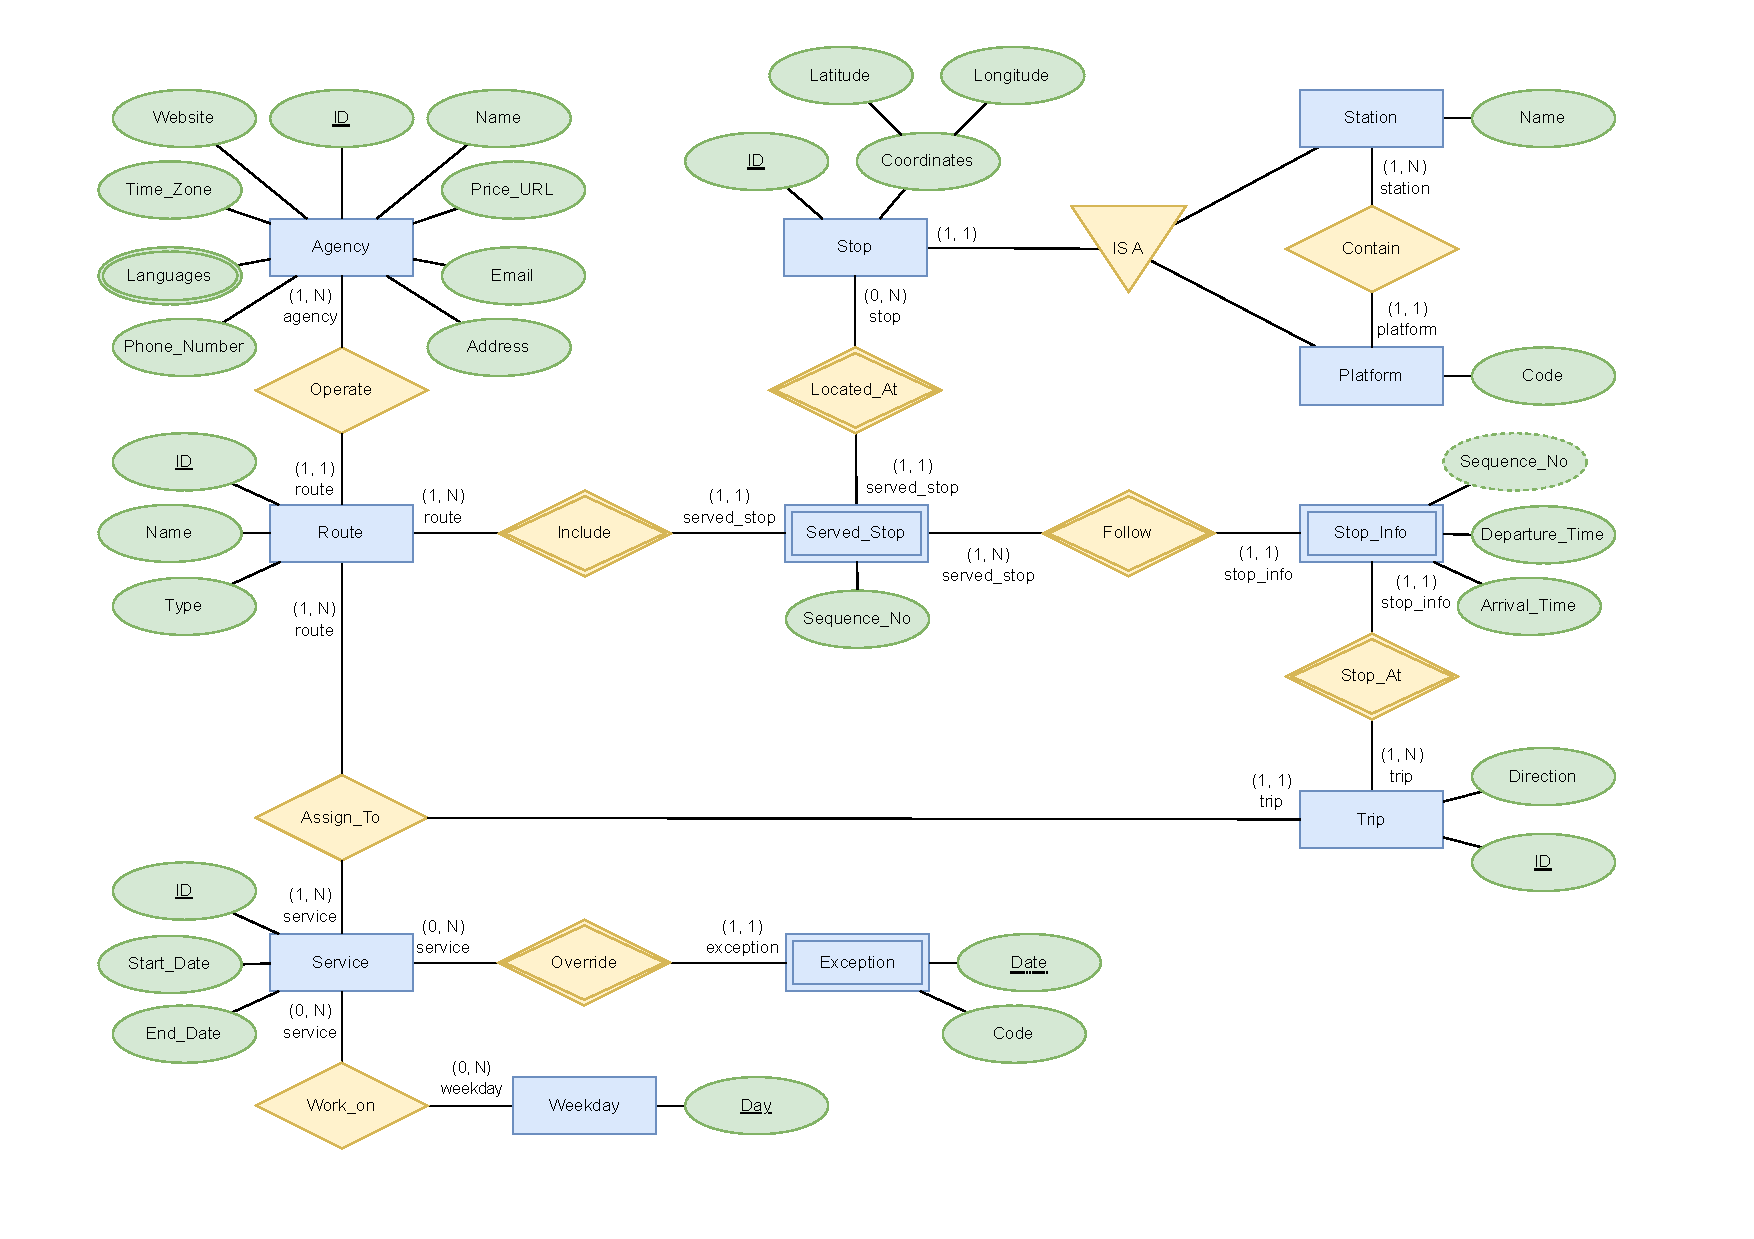
\includegraphics[width=1\linewidth]{./resources/figures/_final_project1_2025-03-14-Final.drawio.pdf}
    \caption{The proposed entity-relationship diagram.}
    \label{fig:ERD}
\end{figure}
\end{landscape}

\section*{Overview}

The train schedule management system aims to provide a centralized, structured way to store, manage, and retrieve information about railway schedules. The system handles main components such as agencies, routes, stops, trips, and services while ensuring data integrity. This project provides the entity-relationship diagram, relational schema, integrity constraints, and normalization process to design a database for managing railway schedules.

\section{Entity-relationship diagram (ERD)} \label{sec:1}

Our proposed entity-relationship diagram for this project is shown in Fig. \ref{fig:ERD}. Below is the justification and some assumptions.

\begin{itemize}
    \item Agency
    \begin{itemize}
        \item Represents an organization that operates railway services.
    \end{itemize}

    \item Route
    \begin{itemize}
        \item Represents a sequence of stops that define a service's path.
        \item Each Route belongs to exactly one Agency, but each Agency can operate multiple Routes. \texttt{(1, N) Agency $\to$ (1, 1) Route (Operate)}.
        \item The combination of Name and Type must be unique.
    \end{itemize}

    \item Stop
    \begin{itemize}
        \item Represents a physical location where trains pick up or drop off passengers.
        \item Specialization (IS A Hierarchy): A Stop must be either a Station or a Platform, but cannot be both simultaneously. \texttt{(1, 1) Stop $\to$ \{Station, Platform\}}.
    \end{itemize}


    \item Station/Platform
    \begin{itemize}
        \item A Station contains multiple Platforms, and each Platform belongs to exactly one Station (assumption). \texttt{(1, N) Station $\to$ (1, 1) Platform (Contain)}.
    \end{itemize}

    \item Served\_Stop
    \begin{itemize}
        \item Represents a stop assigned to a route.
        \item Sequence\_No must start at 1 and increment without gaps.
        \item A route must have at least two stops to be meaningful. In other words, a Route must have at least two Served\_Stops to be valid. \texttt{(2, N) Route → (1, 1) Served\_Stop (Include)}.
        \item Each Served\_Stop must refer to a Stop, but a Stop may exist without being part of a Route (assumption). \texttt{(0, N) Stop $\to$ (1, 1) Served\_Stop (Located\_At)}.
    \end{itemize}

    \item Trip
    \begin{itemize}
        \item Represents a scheduled instance of a route for a service.
        \item A Route can have multiple Trips, but each Trip belongs to one Route. A Service can include multiple Trips, but each Trip belongs to exactly one Service. Therefore, a ternary relationship is formed \texttt{(Assign\_To)}.
    \end{itemize}

    \item Stop\_Info
    \begin{itemize}
        \item Represents actual stop timing for a specific trip.
        \item Each Trip has detailed stop information stored in Stop\_Info. \texttt{(2, N) Trip $\to$ (1, 1) Stop\_Info (Stop\_At)}.
        \item Sequence\_No is derived from Served\_Stop.Sequence\_No and Trip.Direction.
    \end{itemize}

    \item Service
    \begin{itemize}
        \item Represents recurring schedules for trips.

    \end{itemize}

    \item Exception
    \begin{itemize}
        \item Represents deviations from regular service schedules.
        \item Not all Services will have exceptions, but each exception must reference a valid Service (assumption). \texttt{(0, N) Service → (1, 1) Exception (Override)}.
    \end{itemize}

    \item Weekday
    \begin{itemize}
        \item Represents days in a week.
        \item A Service may apply to multiple weekdays, and a weekday may have multiple assigned services. In the ERD, we assume that there may be a day in a week that does not witness a service, and there may be a service that does not run on any day. \texttt{(0, N) Service $\to$ (0, N) Weekday (Work\_On)}.
    \end{itemize}

\end{itemize}

\section{Attribute domains} \label{sec:2}
% non-empty strings
\textbf{Agency}
\begin{itemize}
    \item dom(Agency.ID) = alphanumeric
    \item dom(Agency.Name) = non-empty string
    \item dom(Agency.Website) = non-empty string (URL)
    \item dom(Agency.Time\_Zone) = non-empty string (standard timezone format)
    \item dom(Agency.Languages) = non-empty 2-letter string follow the ISO 639-1 codes (e.g., "fr", "en")
    \item dom(Agency.Phone\_Number) = alphanumeric
    \item dom(Agency.Price\_URL) = non-empty string (URL)
    \item dom(Agency.Email) = non-empty string (email address) $\cup$ \{null\}
    \item dom(Agency.Address) = non-empty string
\end{itemize}

\textbf{Route}
\begin{itemize}
    \item dom(Route.ID) = $\mathbb{N}^+$
    \item dom(Route.Name) = non-empty string
    \item dom(Route.Type) = non-empty string (e.g., "IC", "S", etc.)
\end{itemize}

\textbf{Stop}
\begin{itemize}
    \item dom(Stop.ID) = alphanumeric
    \item dom(Stop.Latitude) = $\{x \in \mathbb{R} \mid -90 \leq x \leq 90\}$ % float (-90 to 90)
    \item dom(Stop.Longitude) = $\{x \in \mathbb{R} \mid -180 \leq x \leq 180\}$ % float (-180 to 180)
\end{itemize}

\textbf{Station}
\begin{itemize}
    \item dom(Station.Name) = non-empty string
\end{itemize}

\textbf{Platform}
\begin{itemize}
    \item dom(Platform.Code) = alphanumeric (e.g., "1", "2b", "C")
\end{itemize}

\textbf{Served\_Stop}
\begin{itemize}
    \item dom(Served\_Stop.Sequence\_No) = $\mathbb{N}^+$
\end{itemize}

\textbf{Trip}
\begin{itemize}
    \item dom(Trip.ID) = alphanumeric
    \item dom(Trip.Direction) = $\{0, 1\}$
\end{itemize}

\textbf{Stop\_Info}
\begin{itemize}
    \item dom(Stop\_Info.Sequence\_No) = $\mathbb{N}^+$
    \item dom(Stop\_Info.Departure\_Time) = date/time $\cup$ \{null\}
    \item dom(Stop\_Info.Arrival\_Time) = date/time $\cup$ \{null\}
\end{itemize}

\textbf{Service}
\begin{itemize}
    \item dom(Service.ID) = alphanumeric
    \item dom(Service.Start\_Date) = date (e.g. follows the form DD/MM/YYYY)
    \item dom(Service.End\_Date) = date (e.g. follows the form DD/MM/YYYY)
\end{itemize}

\textbf{Weekday}
\begin{itemize}
    \item dom(Weekday.Day) = non-empty string (e.g., "Monday", "Tuesday")
\end{itemize}

\textbf{Exception}
\begin{itemize}
    \item dom(Exception.Date) = date
    \item dom(Exception.Code) = $\{1, 2\}$ % integer (1 = added, 2 = removed)
\end{itemize}

\newpage

\section{Description of non-visible integrity constraints} \label{sec:3}
\begin{itemize}
    \item Agency.Languages has at least one value.
    
    \item Route links at least two Served\_Stops.
    \item Combination of (Route.name, Route.type) is unique.

    \item Stop cannot be both a Station and a Platform simultaneously.
    \item Platform.Code is unique within each Station.

    \item Served\_Stop.Sequence\_No must be strictly increasing within each Route.

    % \item Each Trip must include all Served\_Stops in its assigned Route.

    \item Stop\_Info.Departure\_Time $\geq$ Stop\_Info.Arrival\_Time (except for the first stop in Trip)
    \item Stop\_Info.Arrival\_Time must be NULL for the first Served\_Stop in a Trip.
    \item Stop\_Info.Departure\_Time must be NULL for the last Served\_Stop in a Trip.
    
    \item Service.Start\_Date $\leq$ Exception.Date $\leq$ Service.End\_Date
    \item Service.Start\_Date $\leq$ Service.End\_Date
    \item If a Service has an Exception.Date with Exception.Code = 2 (removal), then there must exist another (exception) Service with the same Exception.Date where Exception.Code = 1 (addition). % Ensuring That If a Service is Removed (Exception_Code = 2), There Must be Another Service Added (Exception_Code = 1) on the Same Date
\end{itemize}

\section{Keys} \label{sec:4}
% This part is based on Excercise 2 TP2
\subsection{Entity}
\begin{itemize}
    \item {Agency}: ID
    \item {Route}: ID
    \item {Stop}: ID
    \item {Trip}: ID
    \item {Service}: ID
    \item {Station}: ID (inherits from Stop)
    \item {Platform}: ID (inherits from Stop)
    \item {Weekday}: Day
    
    \item {Route\_Service}: role "route" of "Operate\_On" + role "service" of "Schedule"
    
    \item {Served\_Stop}: role "route" of "Include" + role "stop" of "Located\_At" 
    \item {Stop\_Info}: role "served\_stop" of "Follow" + role "trip" of "Stop\_At"
    
    \item {Exception}: Date + role "service" of "Override"
\end{itemize}

\subsection{Relationship}
\begin{itemize}
    \item {Operate}: role "route"
    \item {Include}: role "served\_stop"
    \item {Located\_At}: role "coordinates"
    \item {Follow}: role "stop\_info"
    \item {Stop\_At}: role "stop\_info"
    \item {Assign\_To}: role "trip"
    \item {Operate\_On}: role "route\_service"
    \item {Schedule}: role "route\_service"
    \item {Override}: role "exception"
    \item {Work\_On}: role "service" + role "weekday"
    \item {Contain}: role "platform"
    % \item {IS-A}: role "stop" is a specialization of "Stop"  \textcolor{red}{!!! I don't know }
\end{itemize}

\section{Reduction to the relational model} \label{sec:5}
% \subsection{Entity}
\begin{itemize}
    \item \texttt{Agency(\underline{ID\_agency}, Name\_agency, Website, Time\_Zone, Phone\_Number, Price\_URL, Email, Address)}
    \item \texttt{Languages(\underline{ID\_agency}, \underline{Language})}
    \item \texttt{Route(\underline{ID\_route}, Name\_route, Type\_route, ID\_agency)}
    \item \texttt{Stop(\underline{ID\_stop}, Latitude, Longitude)}
    \item \texttt{Station(\underline{ID\_stop}, Name\_station)}
    \item \texttt{Platform(\underline{ID\_stop}, Code\_platform, ID\_stop\_station)}
    \item \texttt{Served\_Stop(\underline{ID\_route}, \underline{ID\_stop}, Sequence\_No\_served\_stop)}
    \item \texttt{Trip(\underline{ID\_trip}, Direction, ID\_route, ID\_service)}
    \item \texttt{Stop\_Info(\underline{ID\_route}, \underline{ID\_stop}, \underline{ID\_trip}, Arrival\_Time, Departure\_Time)} % Sequence_No is a derive attribute   
    \item \texttt{Service(\underline{ID\_service}, Start\_Date, End\_Date)}
    % \item \texttt{Route\_Service(\underline{ID\_route}, \underline{ID\_service})} % REMOVED
    \item \texttt{Exception(\underline{ID\_service}, \underline{Date}, Code\_exception)}
    \item \texttt{Weekday(\underline{Day})}

    \item \texttt{Work\_On(\underline{ID\_exception}, \underline{ID\_service})} % We only consider the many-to-many relationship, other one-to-many relationships are absorbed into then entity having the role of (1, 1)
\end{itemize}

% \begin{itemize}
%     \item \textbf{Agency} (\underline{ID\_agency}, Name\_agency, Website, Time\_Zone, Languages, Phone\_Number, Price\_URL, Email, Address)
%     \item \textbf{Route} (\underline{ID\_route}, Name\_route, Type\_route, ID\_agency)
%     \item \textbf{Stop} (\underline{ID\_stop}, Latitude, Longitude)
%     \item \textbf{Station} (\underline{ID\_stop}, Name\_station)
%     \item \textbf{Platform} (\underline{ID\_stop}, Code\_platform)
    
%     \item \textbf{Served\_Stop} (\underline{ID\_stop, ID\_route}, Sequence\_No\_served\_number)
%     \item \textbf{Trip} (\underline{ID\_trip}, Direction)
%     \item \textbf{Stop\_Info} (\underline{ID\_stop, ID\_route, ID\_trip}, Arrival\_Time, Departure\_Time)
%     \item \textbf{Service} (\underline{ID\_service}, Start\_Date, End\_Date)
%     \item \textbf{Route\_Service} (\underline{ID\_route, ID\_service})
%     \item \textbf{Exception} (\underline{ID\_service, Date\_exception}, Code\_exception)
%     \item \textbf{Weekday} (\underline{Day\_weekday})
% \end{itemize}

% \subsection{Relation}
% \begin{itemize}
%     \item \textbf{Work\_On} (\underline{ID\_service, Day\_weekday}) 
%     \item \textbf{Operate} (\underline{ID\_route}, ID\_agency ) %M-to-1 relation so route can absorb it but not sure if we should do it
%     \item \textbf{Include} (\underline{ID\_route, ID\_stop})%can be absorbed by Served_Stop
%     \item \textbf{Follow} (\underline{ID\_route, ID\_stop, ID\_trip})%can be absorbed by stop_info
%     \item \textbf{Stop\_At} (\underline{ID\_route, ID\_stop, ID\_trip})%can be absorbed by stop_info
%     \item \textbf{Assign\_To} (\underline{ID\_trip}, ID\_route, ID\_service)%can be absorbed by Trip (need to add id_route and id_service to Trip)
%     \item \textbf{Operate\_On} (\underline{ID\_route, ID\_service}) %can be absorbed by Route_Service
%     \item \textbf{Schedule} (\underline{ID\_service, ID\_route})%can be absorbed by Route_Service
%     \item \textbf{Override} (\underline{Date\_exception, ID\_service})%can be absorbed by Exception
%     \item \textbf{located\_at} (\underline{ID\_stop, ID\_route})%can be absorbed by Served_stop
%     \item \textbf{Contain} (\underline{ID\_stop})
% \end{itemize}

\newpage

\section{Analysis of normal forms} \label{sec:6}

\subsection{\texttt{Agency(\underline{ID\_agency}, Name\_agency, Website, Time\_Zone, Phone\_Number, Price\_URL, Email, Address)}}

\textbf{Non-trivial functional dependency:}
\begin{itemize}
    \item \{ID\_agency\} $\rightarrow$ \{Name\_agency, Website, Time\_Zone, Phone\_Number, Price\_URL, Email, Address\}
\end{itemize}

\textbf{Candidate key:}
\begin{itemize}
    \item \{ID\_agency\}
\end{itemize}

\textbf{Normal form analysis:}
\begin{itemize}
    \item \textbf{1NF:} Satisfied - All attributes contain only atomic, non-repetitive values that are constant over time.
    
    \item \textbf{2NF:} Satisfied - The primary key is a single attribute, so there cannot be any partial dependencies.
    
    \item \textbf{3NF:} Satisfied - All non-key attributes depend only on the candidate key \{ID\_agency\} and not on other non-key attributes.
    
    \item \textbf{BCNF:} Satisfied - The only determinant \{ID\_agency\} is a candidate key, meaning all determinants are superkeys.
\end{itemize}

\subsection{\texttt{Languages(\underline{ID\_agency}, \underline{Language})}}
\textbf{Non-trivial functional dependency:}
\begin{itemize}
    \item There are no non-trivial functional dependencies in this relation since all attributes are part of the primary key.
\end{itemize}
\textbf{Candidate key:}
\begin{itemize}
    \item \{ID\_agency, Language\}
\end{itemize}

\textbf{Normal form analysis:}
\begin{itemize}
    \item \textbf{BCNF:} Satisfied -  All attributes form part of the primary key, thus, there are no non-key attributes that could create problematic functional dependencies.
\end{itemize}

\subsection{\texttt{{Route}(\underline{ID\_route}, Name\_route, Type\_route, ID\_agency)}}
\textbf{Non-trivial functional dependencies:}
\begin{itemize}
    \item \{ID\_route\} $\rightarrow$ \{Name\_route, Type\_route, ID\_agency\}
    \item \{Name\_route, Type\_route\} $\rightarrow$ \{ID\_route, ID\_agency\}
\end{itemize}

\textbf{Candidate keys:}
\begin{itemize}
    \item \{ID\_route\}
    \item \{Name\_route, Type\_route\}
\end{itemize}

\textbf{Normal form analysis:}
\begin{itemize}
    \item \textbf{1NF:} Satisfied - All attributes contain only atomic, non-repetitive values that are constant over time.
    
    \item \textbf{2NF:} Satisfied - The primary key is a single attribute, so there cannot be any partial dependencies.
    
    \item \textbf{3NF:} Satisfied - All non-key attributes depend only on the candidate key \{ID\_route\} and not on other non-key attributes.
    
    \item \textbf{BCNF:} Satisfied - \{ID\_route\} is a candidate key and \{Name\_route, Type\_route\} is a superkey, meaning all determinants are superkeys.
\end{itemize}

\subsection{\texttt{{Stop}(\underline{ID\_stop}, Latitude, Longitude)}}
\textbf{Non-trivial functional dependency:}
\begin{itemize}
    \item \{ID\_stop\} $\rightarrow$ \{Latitude, Longitude\}
\end{itemize}

\textbf{Candidate key:}
\begin{itemize}
    \item \{ID\_stop\}
\end{itemize}

\textbf{Normal form analysis:}
\begin{itemize}
    \item \textbf{1NF:} Satisfied - All attributes contain only atomic, non-repetitive values that are constant over time.
    
    \item \textbf{2NF:} Satisfied - The primary key is a single attribute, so there cannot be any partial dependencies.
    
    \item \textbf{3NF:} Satisfied - All non-key attributes depend only on the candidate key \{ID\_stop\} and not on other non-key attributes.
    
    \item \textbf{BCNF:} Satisfied - The only determinant \{ID\_stop\} is a candidate key, meaning all determinants are superkeys.
\end{itemize}

\subsection{\texttt{{Station}(\underline{ID\_stop}, Name\_station)}}
\textbf{Non-trivial functional dependency:}
\begin{itemize}
    \item \{ID\_stop\} $\rightarrow$ \{Name\_station\}
\end{itemize}

\textbf{Candidate key:}
\begin{itemize}
    \item \{ID\_stop\}
\end{itemize}

\textbf{Normal form analysis:}
\begin{itemize}
    \item \textbf{1NF:} Satisfied - All attributes contain only atomic, non-repetitive values that are constant over time.
    
    \item \textbf{2NF:} Satisfied - The primary key is a single attribute, so there cannot be any partial dependencies.
    
    \item \textbf{3NF:} Satisfied - All non-key attributes depend only on the candidate key \{ID\_stop\} and not on other non-key attributes.
    
    \item \textbf{BCNF:} Satisfied - The only determinant \{ID\_stop\} is a candidate key, meaning all determinants are superkeys.
\end{itemize}
\subsection{\texttt{{Platform}(\underline{ID\_stop}, Code\_platform, ID\_stop\_station)}}
\textbf{Non-trivial functional dependency:}
\begin{itemize}
    \item \{ID\_stop\}$\rightarrow$ \{Code\_platform, ID\_stop\_station\}
\end{itemize}

\textbf{Candidate key:}
\begin{itemize}
    \item \{ID\_stop\}
\end{itemize}

\textbf{Normal form analysis:}
\begin{itemize}
    \item \textbf{1NF:} Satisfied - All attributes contain only atomic, non-repetitive values that are constant over time.
    
    \item \textbf{2NF:} Satisfied - The primary key is a single attribute, so there cannot be any partial dependencies.
    
    \item \textbf{3NF:} Satisfied - All non-key attributes depend only on the candidate key \{ID\_stop\} and not on other non-key attributes.
    
    \item \textbf{BCNF:} Satisfied - The only determinant \{ID\_stop\} is a candidate key, meaning all determinants are superkeys.
\end{itemize}

\subsection{\texttt{{Served\_Stop} (\underline{ID\_route}, \underline{ID\_stop}, Sequence\_No\_served\_stop)}}
\textbf{Non-trivial functional dependency:}
\begin{itemize}
    \item \{ID\_route, ID\_stop\} $\rightarrow$ \{Sequence\_No\_served\_stop\}
\end{itemize}

\textbf{Candidate key:}
\begin{itemize}
    \item \{ID\_route, ID\_stop\}
\end{itemize}

\textbf{Normal form analysis:}
\begin{itemize}
    \item \textbf{1NF:} Satisfied - All attributes contain only atomic, non-repetitive values that are constant over time.
    
    \item \textbf{2NF:} Satisfied - Sequence\_No\_served\_stop is fully dependent on the key \{ID\_route, ID\_stop\}.
    
    \item \textbf{3NF:} Satisfied - All non-key attributes depend only on the candidate key \{ID\_route, ID\_stop\} and not on other non-key attributes.
    
    \item \textbf{BCNF:} Satisfied - The only determinant \{ID\_route, ID\_stop\} is a candidate key, meaning all determinants are superkeys.
\end{itemize}
\subsection{\texttt{{Trip}(\underline{ID\_trip}, Direction, ID\_route, ID\_service)}}
\textbf{Non-trivial functional dependency:}
\begin{itemize}
    \item \{ID\_trip\} $\rightarrow$ \{Direction, ID\_route, ID\_service\}
\end{itemize}

\textbf{Candidate key:}
\begin{itemize}
    \item \{ID\_trip\}
\end{itemize}

\textbf{Normal form analysis:}
\begin{itemize}
    \item \textbf{1NF:} Satisfied - All attributes contain only atomic, non-repetitive values that are constant over time.
    
    \item \textbf{2NF:} Satisfied - The primary key is a single attribute, so there cannot be any partial dependencies.
    
    \item \textbf{3NF:} Satisfied - All non-key attributes depend only on the candidate key \{ID\_trip\} and not on other non-key attributes.
    
    \item \textbf{BCNF:} Satisfied - The only determinant \{ID\_trip\} is a candidate key, meaning all determinants are superkeys.
\end{itemize}

\subsection{\texttt{{Stop\_Info}(\underline{ID\_route}, \underline{ID\_stop}, \underline{ID\_trip}, Arrival\_Time, Departure\_Time)}}
\textbf{Non-trivial functional dependency:}
\begin{itemize}
    \item \{ID\_route, ID\_stop, ID\_trip\} $\rightarrow$ \{Arrival\_Time, Departure\_Time\}
\end{itemize}

\textbf{Candidate key:}
\begin{itemize}
    \item \{ID\_route, ID\_stop, ID\_trip\}
\end{itemize}

\textbf{Normal form analysis:}
\begin{itemize}
    \item \textbf{1NF:} Satisfied - All attributes contain only atomic, non-repetitive values that are constant over time.
    
    \item \textbf{2NF:} Satisfied - Arrival\_Time and Departure\_Time are fully dependent on the key \{ID\_route, ID\_stop, ID\_trip\}.
    
    \item \textbf{3NF:} Satisfied - All non-key attributes depend only on the candidate key \{ID\_route, ID\_stop, ID\_trip\} and not on other non-key attributes.
    
    \item \textbf{BCNF:} Satisfied - The only determinant \{ID\_route, ID\_stop, ID\_trip\} is a candidate key, meaning all determinants are superkeys.
\end{itemize}

\subsection{\texttt{{Service}(\underline{ID\_service}, Start\_Date, End\_Date)}}
\textbf{Non-trivial functional dependency:}
\begin{itemize}
    \item \{ID\_service\} $\rightarrow$ \{Start\_Date, End\_Date\}
\end{itemize}

\textbf{Candidate key:}
\begin{itemize}
    \item \{ID\_service\}
\end{itemize}

\textbf{Normal form analysis:}
\begin{itemize}
    \item \textbf{1NF:} Satisfied - All attributes contain only atomic, non-repetitive values that are constant over time.
    
    \item \textbf{2NF:} Satisfied - The primary key is a single attribute, so there cannot be any partial dependencies.
    
    \item \textbf{3NF:} Satisfied - All non-key attributes depend only on the candidate key \{ID\_service\} and not on other non-key attributes.
    
    \item \textbf{BCNF:} Satisfied - The only determinant \{ID\_service\} is a candidate key, meaning all determinants are superkeys.
\end{itemize}

\subsection{\texttt{{Route\_Service}(\underline{ID\_route}, \underline{ID\_service})}}
\textbf{Non-trivial functional dependency:}
\begin{itemize}
    \item There are no non-trivial functional dependencies in this relation since all attributes are part of the primary key.
\end{itemize}
\textbf{Candidate key:}
\begin{itemize}
    \item \{ID\_route, ID\_service\}
\end{itemize}

\textbf{Normal form analysis:}
\begin{itemize}
    \item \textbf{BCNF:} Satisfied -  All attributes form part of the primary key, thus, there are no non-key attributes that could create problematic functional dependencies.
\end{itemize}
\subsection{\texttt{{Exception}(\underline{ID\_service}, \underline{Date}, Code\_exception)}}
\textbf{Non-trivial functional dependency:}
\begin{itemize}
    \item \{ID\_service, Date\} $\rightarrow$ \{Code\_exception\}
\end{itemize}

\textbf{Candidate key:}
\begin{itemize}
    \item \{ID\_service, Date\}
\end{itemize}

\textbf{Normal form analysis:}
\begin{itemize}
    \item \textbf{1NF:} Satisfied - All attributes contain only atomic, non-repetitive values that are constant over time.
    
    \item \textbf{2NF:} Satisfied - Date is fully dependent on the key \{ID\_service, Date\}.
    
    \item \textbf{3NF:} Satisfied - All non-key attributes depend only on the candidate key \{ID\_service, Date\} and not on other non-key attributes.
    
    \item \textbf{BCNF:} Satisfied - The only determinant \{ID\_service, Date\} is a candidate key, meaning all determinants are superkeys.
\end{itemize}

\subsection{\texttt{{Weekday}(\underline{Day})}}
\textbf{Non-trivial functional dependency:}
\begin{itemize}
    \item There are no non-trivial functional dependencies in this relation since all attributes are part of the primary key.
\end{itemize}
\textbf{Candidate key:}
\begin{itemize}
    \item \{Day\}
\end{itemize}

\textbf{Normal form analysis:}
\begin{itemize}
    \item \textbf{BCNF:} Satisfied -  All attributes form part of the primary key, thus, there are no non-key attributes that could create problematic functional dependencies.
\end{itemize}
\subsection{\texttt{{Work\_On}(\underline{ID\_exception}, \underline{ID\_service})}}
\textbf{Non-trivial functional dependency:}
\begin{itemize}
    \item There are no non-trivial functional dependencies in this relation since all attributes are part of the primary key.
\end{itemize}
\textbf{Candidate key:}
\begin{itemize}
    \item \{ID\_exception, ID\_service\}
\end{itemize}

\textbf{Normal form analysis:}
\begin{itemize}
    \item \textbf{BCNF:} Satisfied -  All attributes form part of the primary key, thus, there are no non-key attributes that could create problematic functional dependencies.
\end{itemize}
% \section*{Conclusion}


% \newpage

% \printbibliography

% \newpage

% \appendix

% \renewcommand\thefigure{\thesection.\arabic{figure}}    
% \renewcommand\thetable{\thesection.\arabic{table}} 

% \section{Appendix} \label{appendix}

% \setcounter{figure}{0}
% \setcounter{table}{0}

\end{document}